\section{Architektur}
Es wird die während des Entwicklungsprozess entstandene Architektur von helios beschreiben.


\begin{figure*}[t]
    \centering
    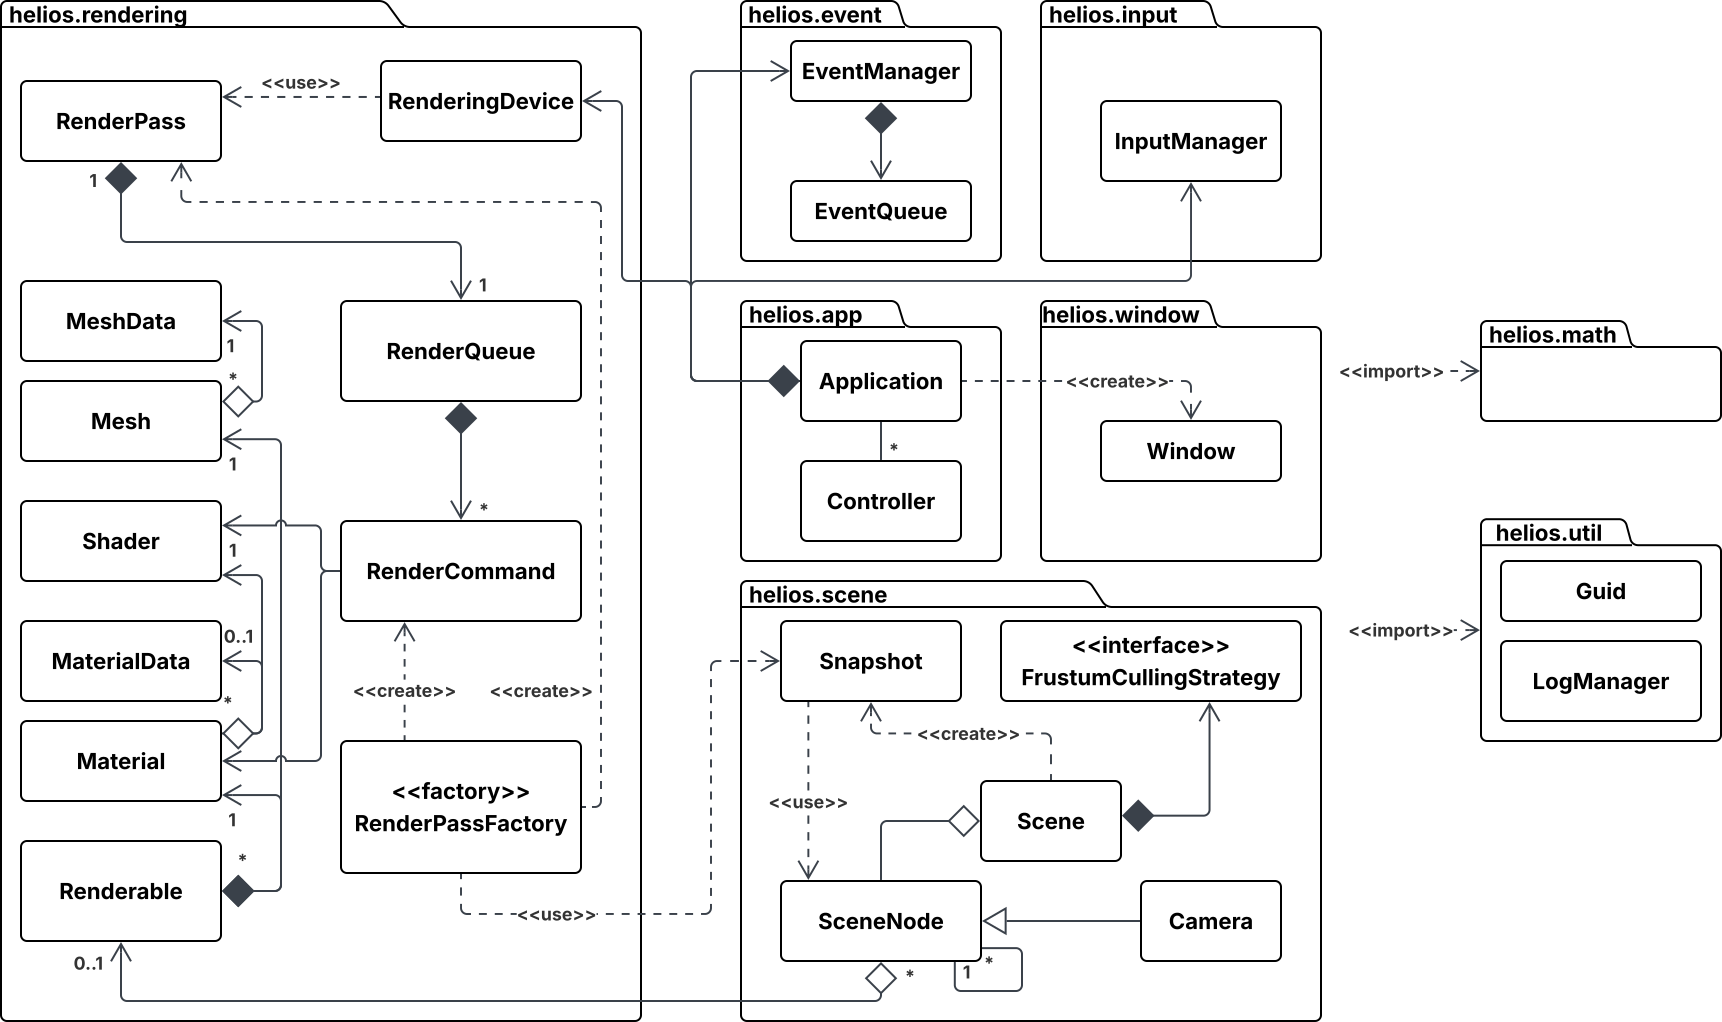
\includegraphics[width=1\textwidth]{img/package_diagram.svg}% \linewidth == Spaltenbreite
    \caption{Render-Pipeline-Übersicht.}
    \label{fig:pipeline}
\end{figure*}



und  \texttt{glfw}, oder die Implementierung des OpenGL-Rendering-Backends auf Basis von \texttt{glad}.

Die Grungdlegende Architektur von Helios kann derzeigt in folgende gliedert sich wie folgt:

\begin{verbatim}
    Applikationsschicht
        EventVerabeitung
        InputVerarbeitung
        GameSystem - Physik, NPC, Spieler (soft Architecture, [RM04] Game Architecture and Design - A New Edition, 612)
        Scene
        RenderingSystem
\end{verbatim}

Wir verstehen hierbei die Auftrennung von Applikation und Game Engine wie folgt: Eine SApplikation hostet die Game Engine und stellt Ressourcen zur Verfügung, damit die Game Engine Eingaben in Form von Commands erhält, diese entsprechend ihrer internenen Logik verarbeitet, Game Objekte aktualisieren kann und als Ausgabe an das RenderingSytem weitergibt - für die Applikation stellt das GameSystem in dieser Hinsicht eine BlackBox dar, deren interne Implementierung nicht bekannt ist und zunächst Schnitttsellen zur Eingabe von COmmands erhält. Bekkannt ist nur, das in jedem Frame eine Aktualisierung der von der Game Engine repräsentierten Spielewelt stattfinden soll.

\subsection{Applikationsschicht}
ordner: app
Wir haben für ein Spiel ein Applikationsklasse vorgesehen, wie sie auch üblicherwiese aus der GUI Programmierung bekannt ist. Hierbei stellt eine Applikatiosnklasse eine Shell dar, die den Zugriff auf alle Subsytemse kapselt und die Kommunikation und STeuerung der Sunbsysteme übernimmt und vermittelt.
HIerzu erlauben wir die Verwendung von ApplikationsControllern, die bei der Anwendung registeriert, auf bestimmte Ergeignise der EventQueue reagiert und entsprechende Aktionen ausführen kann.

\subsection{InputVerarbeitung}
ordner: input
Die Inputverarbeitung wird über einen InputManager realisiert, der an ein Anwendungsfenster gebunden Ereignisse überacht wie Tastatureingaben. Hierzu findet ein Polling zu Beginn der Game Loop statt, die die Ereignisse sammelt und dem InputManager über entsprechende InputAdapter due APIs anbindet, die für die Abstraktion der nativen Ereignisse zuständig sind (glfw).
Geplant ist, aus der Inpztverabbeitung entsprechende Commands zu generieren, die an das GameSystem weitergelitet werden.

\subsection{EventVerarbeitung}
Ordner: event
Zur Steuerung des Fenster haben wir einen Eeinfachen EventManager implementiert, der über post Events in eine EventQueue schreibt, die zu Beginn der Game loop - also noch vor dem Input Manager - Applikationssüpezifische Events and die registrierten Applikationscontroller dispatched. Eine Zusammenführung des InputManagers mit dem EventSystem ist theoretisch möglich, eine Auftrennung in diese beiden Systeme schien aber zunächst aufgrund der noch nicht implementierten InputVErabreitung und die Transformation der Commands für das Game Subsystem nötig, um später nicht an zu vielen Stellen ein Refactoring betreiben zu müssen, sollte sich herausstellen, dass aus Performancegründen die Abarebitung über den EventManager der Applikation nicht sinnvoll ist, und die Inputs auf einer niedrigeren Abstraktionseben arbeiten müssen.

\subsection{Fenster zur Darstellung des Spiels}
ordner: Window
Wir haben eine einfache Abstraktionsschicht erstellt, die zunächst noch recht nah an den von glfw erwarteten Kommandos zur Fenstererzeugung ist. Da die Erfahrung mit anderen Fenstersystemen fehlt, muss beim Einsatz einer anderen ``platform`` hier ggfl. noch ein Refactoring in noch generischere Klasse erfolgen.

\subsection{Utility Klassen}
ordner: util
Beinhaltet ein Modul, das Logginfunktionalität bereitstsellt, sowie eine Threadsicher Implementierung einer Guid (global unique identifier), die für Entitären wie SceneNodes zur eindeutigen Identtifizierung verwendet werden kann. log ausweichen auf spdlog

\subsection{Mathematische Typen und Operationen}
ordner math
Beinhaltet die für die Transformation der Szenen-Objekte benötigten mathematischen Typen wie Vektoren und Matrizen sowie Operationen zur Transformation der Geometrie der einzelnen Objekte, bspw. Rotatiosnmatrizen, Schereung und TRanslation. Für helios haben wir uns zunächst gegen die Verwendung von den bekannten Mathematik-Bibliotheken entschieden, um den Lernprozess zu fördern und Erfahrung zu sammeln im BEreich performancektirischer Anwendungen und möglichst optimaler Implementierung mathematischer Operationen auf einem höheren Abstraktionsgrad, alsu zunächst ohne explizite Compileroptimierungen wie sdim.\\
Die Schnottstellen sind aber angelehnt an den bekannten mathematik bibliotheken, weshalb sich Entwickler hier schnell zurecht finden sollten.

\subsection{Szenengraph}
Der Szenengraph in Helios orientiert sich an den gängigen Empfehlungen zur Implementierung eines solchen. Die Klasse Scene ist so implementiert, dass sie einen impliziten root-Knoten besitzt, der eine beliebige Anzahl von Kindknoten besitzen kann, welche wiederum Teilbäume in dem Sezene repräsentieren. Jeder SceneNode besitzt eine Transform-Instanz, die seine lokales Modell repräsentiert und entsprechend der übergeordneten Knoten bei der Berechnung der WorldTransformation die Daten der Elternknoten mit in die Berechnung einbezieght.\\
SceneNodes können darstellbar sein oder Meta-Szeneknoten wie Kameras repräsentieren, die wiederum keine Kindknoten erlauben, aber als Blätetr in einem Teilbaum bspw. als bewegliche Kamera verwendet werden können.\\
Eine Szene kann also beliebig viele Kameras beinhalten, so dass es bspw. möglich ist, eine Spielsituation gleichzeitig aus verschiedenen Blickwinkeln zu betrachten.\\
Darstellbare Szeneknoten werden beim Culling berücksichtigt, die wir in der abstrakten Klasse FrustumCullingStrategy als Vertrag veinbaren und mit der wir eine Szenen-Instanz konfigurieren.\\
Die Application Stage ((Application Stage [Gre19, 687]).) der Rendering Pipeline betreten wir mit der Fassaden-Methode snapshot(helios::scene::Camera& camera) erstellt dann auf Basis der viewMatrix und Projektionsmatrix der referenzierten Camera ein Culling und liefert alle im sichtbaren Bereich befindlichen SceneNodes als SnapshotItems in einer flachen liste zurück. Diese Snapshots sind dann Basis zur Erstellung des RenderPasses, der an die Renderpipeline wie im nachfolgenden Abschnitt beschrieben übergeben wird. LIghtNodes, um einem spieler zu folgen etc

\subsection{Render Pipeline}
Ordner: rendering
Das Rendering System befindet sich im Ordner render und ist in verschiedene Teilmodule aufgeteilt, u.a. asset, dass Vertex und Index-Daten für verschiedene geometrische Figuren beinhaltet, einem Ordner Model, in dem Klassen zur Kapselung von Material und RenderBackend spezifischen Mesh-Daten zur Verfügung stellt sowie einen shader-Ordner, in dem ebenfalls Render spezifische Implementierungen für die Shader vorliegent.\\
Diese Typen werden als Teil einer Aggregation genutzt, die durch Renderable repreäsentiert wird: Ein Renderable ist eine Backend-unabhängige Basisklasse, die einen shared pointer auf eine Mesh-Instanz hält sowie einen unique pointer auf ein Material., welches wiederum einen shared pointer auf Shader beinhaltet und Materialdata.
Damit haben wir zunächst die Möglichkeit geschaffen, Shader MNesh und MaterialData unter den Renderables zu teilen, gleichzeitig können wir über eine MaterialINstanz intsanzspezifische Parameter festlegen (Quelle; außerdem Illustration erstellen mit den Kardinalitäten).\\
Den im vorherigen Abschnitt erwähnten Snapshot übergeben wir an eine RenderPassFactory, die aus dem Snapshot und den enthaltenen Daten einen RenderPass erzeugt. Ein RenderPass enthält eine RenderQueue, die besagte Renderables enthält. Wir hoffen, durch dieses Design später ein optimales vcorortieren der Rednderables erreichen zu können, bevor diese von dem unterliegenden Rendering Backend verabrietet werden ([https://realtimecollisiondetection.net/blog/?p=86]).\\
Ein Render Pass - von dem es theoretisch beliebig viele ausprägungen gibt, und der für den derzeitigen Renderpass benötigte Informationen wie die view und projektionsmatrix für die shader uniforms beinhaltet, wird dann an das RenderDevice übergeben, das mit der Applikation konfiguriert und in einem FensterContext erstellt wurde. In einer pre, do und post Methode wird der Renderpass dann abgerabeitet und die Daten in den entsprechenfd aktiven Fensterbuffer geschrieben, zu dem am Ender der main loop dann umgeschaltet wird.

ForwardRendering, Deferred Rendering, Memory Allocations langsam, arbeiten mit vector, eine ausnahme aray mit sentinel, Data Driven Programming explici array, minimize vtable lookups, cache firendly, branch predicting as possible
